\documentclass[parskip]{scrartcl}
\usepackage[utf8]{inputenc}
\usepackage[ngerman]{babel}
\usepackage[round]{natbib}
%\usepackage{color} % used for comments
\usepackage{listings}
\usepackage{url}
\usepackage{booktabs}
\usepackage{array}
\usepackage{courier}
\usepackage[htt]{hyphenat}
\usepackage{graphicx}
\lstset {
  language=xml,
  basicstyle={\footnotesize\ttfamily},
  numbers=none,
  aboveskip=5mm,
  belowskip=5mm,
  showstringspaces=false,
  columns=flexible,
  %keywordstyle={\bfseries\color{Blue}},
  %commentstyle={\color{Red}\textit},
  %stringstyle=\color{Magenta},
  frame=single,
  breaklines=true,
  breakatwhitespace=true,
  tabsize=4,
  morekeywords={rdf,rdfs,owl}  % <-- adding custom keywords
}

\begin{document}
\subject{Projektdokumentation im Modul Semantic Web}
\title{Familienfreundlichste Stadtteile der Stadt Leipzig}
\author{Alexander Müller}
\date{10.07.2015}

\maketitle


\paragraph{Recherchefragestellung: }
Welcher ist der familienfreundlichste Stadtteil Leipzigs auf Grund der Anzahl der vorhandenen Schulen, Kindergärten, Spielplätze, Schwimmbäder, Sporthallen und Sportplätze.


\section{Inhaltliche Interpretation der Fragestellung}
Leipzig ist eine wachsende Stadt und hat großes Interesse daran, dass junge Menschen gern in Leipzig leben und will diese bei einer Familiengründung unterstützen. Die Stadt Leipzig ist dabei sehr bemüht attraktiver für Familien zu werden und hat dazu bereits 2011 einen "`Aktionsplan kinder- und familienfreundliche Stadt Leipzig 2011 bis 2015"'\footnote{siehe \url{www.leipzig.de/jugend-familie-und-soziales/familienfreundliche-stadt/}} beschlossen.

Ein Rangliste der Stadtteile nach ihrer Familienfreundlichkeit könnte ein wichtiges Hilfsmittel sein, um zu bestimmen, in welchen Regionen der Stadt noch Handlungsbedarf besteht. Als Kriterium soll dabei die Anzahl der in einem Stadtteil vorhandenen Einrichtungen für Kinder verwendet werden. Die Einrichtungen für Kinder sind im Rahmen dieses Projektes auf Schulen (Grundschulen, Realschulen, Gymnasien), Kindergärten, Spielplätze, Schwimmbäder, Sporthallen und Sportplätze beschränkt.


\section{Relevante Datenquellen}
Für die Auswertung der Fragestellung werden Lageinformationen zu sämtlichen Einrichtungen in Leipzig benötigt. Zusätzlich müssen diese dann den jeweiligen Stadtteilen der Stadt Leipzig zugeordnet werden können. Im Folgenden werden alle dafür relevanten Datenquellen aufgelistet und beschrieben.

\subsection{Datenbasis des Leipzig Data Projekts }
Die Leipziger Initiative für Offene Daten bemüht sich schon seit einigen Jahren um die Etablierung offener Daten in der Leipziger Region. Seit dem wurden verschiedene Daten systematisch erfasst, gepflegt und unter einer freien Lizenz veröffentlicht. Die Datenbasis des Leipzig Data Projekts besteht aus RDF-Wissensbasen für verschiedene Themenbereiche, welche in einem OntoWiki\footnote{siehe \url{http://leipzig-data.de/Data/}} öffentlich inspiziert werden können. Zusammen mit verschiedenen Tools wurden die Wissensbasen zu Verwaltung auch in einem Versionsverwaltungssystem im Turtle-Format\footnote{siehe \url{https://github.com/LeipzigData}} veröffentlicht. Außerdem wird ein Sparql Endpunkt\footnote{siehe \url{http://leipzig-data.de:8890/sparql}} bereitgestellt, um Abfragen auf den Daten auszuführen. Für das Projekt wurden folgende Wissenbasen verwendet:
\begin{itemize}
\setlength{\itemsep}{-3pt}
\item Adressen in der Stadt Leipzig
\item Schulen der Stadt Leipzig
\item Stadtbezirke und Ortsteile
\end{itemize}
Außer diesen sind zum Beispiel Wissensbasen über sämtliche Bürgervereine, Polizeidirektionen, Seniorenbüros, Personen und Geo-Koordinaten für alle Adressen in Leipzig verfügbar.
 

\begin{tabular}{l|p{9cm}}
	Link & \url{http://leipzig-data.de/Data/} \\
 	Datenformat & RDF, OWL \\
 	Schnittstelle & SPARQL, Linked Data \\
 	Lizenz & CC0 1.0 Universal \\
 	Open Data & $\star\star\star\star\star$ \\
\end{tabular}

\subsection{Adressdatenbank auf der Webseite der Stadt Leipzig}
Die Stadt Leipzig bietet auf ihrer Webseite einen Service zur Recherche unterschiedlichster Einrichtungen in Leipzig. Die Datensammlung ist sehr umfangreich und lässt sich nach Themen sowie Gebieten filtern. Vorhandene Themen sind beispielsweise Gesundheit, Kinder, Jugend und Familie, Kulturvereine, Senioren, Sport, Migration, Integration und Interkulturelles, Wissenschaft, Wirtschaft, Kultur, Behinderung und Bildung mit jeweils mehreren unter Kategorien. Über diese Adresssuche wurden folgende Iformationen für das Projekt extrahiert:
\begin{itemize}
\setlength{\itemsep}{-5pt}
\item Kindergärten
\item Spielplätze
\item Schwimmhallen
\item Sportplätze
\item Sporthallen
\end{itemize}

Zu jedem gefunden Eintrag der Adresssuche existiert eine Webseite mit einer Detailansicht des Eintrages. Auf dieser Detailseite werden genauere Informationen zu der bestimmten Einrichtung angezeigt, beispielsweise Kurzbeschreibungen, Adressinformationen, Kontaktmöglichkeiten, Ansprechpartner, Angebote, Bilder oder Öffnungszeiten. Jedoch ist der Umfang der angegeben Informationen sehr unterschiedlich.

\begin{tabular}{l|p{9cm}}
	Link & \url{http://www.leipzig.de/suchergebnisse-adressdatenbank/} \\
 	Datenformat & HTML \\
 	Schnittstelle & HTTP (interne API) \\
 	Lizenz & urheber- bzw. leistungsrechtlich geschützt \\
 	Open Data & $\star\star\star\star$ \\
\end{tabular}


\section{Extraktion relevanter Daten und Import in einen Triplestore }


\subsection{Extraktion Leipzig Data Datenbasis}
Die Extraktion der Daten erfolgt über das OntoWiki Leipzig Data Projekt. Dabei wurden die RDF-Daten der drei Wissensbasen (Adressen, Ortsteile, Schulen der Stadt Leipzig) im Turtle Format exportiert und lokal abgespeichert.

\subsection{Extraktion www.Leipzig.de}\label{extract_leipzig}
Die Extraktion der Daten von der Webseite der Stadt Leipzig war um 
Einiges komplexer, da diese Informationen erst aus den HTML-Seiten extrahiert werden mussten und nicht bereits als Tripel vorgelegen haben.
Zur Extraktion wurde ein Java-Programm geschrieben, welches mit Hilfe der Java-Bibliothek "`JSOUP"'\footnote{siehe \url{http://jsoup.org}} die Daten aus den HTML-Seiten extrahiert. Die Adresssuche auf der Webseite verwendet eine interne API, welche über Parameter der GET-Methode des Hypertext Transfer Protocols (HTTP) die Suchkriterien übergeben bekommt. Welche Parameter übergeben werden können, konnte durch die Analyse des Seitenquelltextes herausgefunden werden. Die folgende URL zeigt einen beispielhaften Aufruf der Suche, bei dem alle Kindergärten angezeigt werden sollen.

\begin{lstlisting}
http://www.leipzig.de/suchergebnisse-dressdatenbank/
   ?tx_ewerkaddressdatabase_pi[showAll]=1
   &tx_ewerkaddressdatabase_pi[topics]=105
   &tx_ewerkaddressdatabase_pi[query]=
   &tx_ewerkaddressdatabase_pi[action]=list
   &tx_ewerkaddressdatabase_pi[controller]=Address
\end{lstlisting}

Über den Parameter "`\texttt{tx\_ewerkaddressdatabase\_pi[topics]}"' wird eine eindeutige Nummer der gesuchten Kategorie übergeben, in dem oberen Beispiel steht die 105 für die Suchkategorie Kindergärten. Die für die Fragestellung relevanten Kategorien und deren Nummern wurden ebenfalls durch die Analyse des Quellcodes der Auswahlbox herausgefunden.

\begin{table}[h]
\label{my-label}
\begin{tabular}{@{}ll@{}}
\toprule
{\bf Kategorie} & {\bf ID} \\ \midrule
Kindergärten    & 105      \\
Spielplätze     & 111      \\
Sporthallen     & 375      \\
Sportplätze     & 377      \\
Schwimmbäder    & 433, 435 \\ \bottomrule
\end{tabular}
\end{table}

Nach Aufruf einer Suchanfrage wird eine HTML-Seite mit einer Ergebnisliste zurückgegeben. Diese Liste enthält die Namen Link zu den Detailseiten der gefundenen Einträge.

Im zweiten Schritt des Java-Programms werden die Detailseiten einzeln aufgerufen, was ebenfalls mit JSOUP realisiert wurde. Da JSOUP das kompletten Document Object Model (DOM) der übergebenen URL lädt, kann über  jedes Element der HTML-Seite genau adressiert und extrahiert werden. Die extrahierten Informationen aus den Detailseiten (Name, URL, Adresse, Stadtteil) werden bei jedem gefundenen Eintrag als Attribute in ein Objekt geschrieben und anschließend das Objekt in einer Liste gespeichert.

Da diese Extraktion sehr zeitaufwendig ist, wird die Liste mit den Objekten für die weitere Verarbeitung im JSON-Format zwischengespeichert.
 

\subsection{Erstellen der RDF-Triple und Import in den Triplestore}
Die im Kapitel \ref{extract_leipzig} extrahierten Daten wurden anschließend mit Hilfe des Jena-Frameworks\footnote{siehe \url{https://jena.apache.org}} in RDF-Daten überführt und gespeichert. Dazu wurde ein Ontologie erstellt, welche aus jeweils einer Klasse für jeder der fünf Kategorien (Kindergärten, Spielplätze, Sporthallen, Sportplätze, Schwimmbäder) besteht. Dabei wurde der private Namespace \url{http://www.imn.htwk-leipzig.de/~amuelle3/Data/} mit dem Präfix \textit{am} verwendet.

Die fünf Klassen ähneln sich sehr in ihren Eigenschaften. Alle Klassen besitzen die Datatype-Property \textit{rdfs:label}, welche die genaue Beschreibung des Objektes enthält. Weiterhin besitzen alle fünf Klassen die Object-Property \textit{ld:inOrtsteil}. Diese Property stammt aus der Leipzig Data Ontologie und der Präfix \textit{ld } steht für folgenden Namespace: \url{http://leipzig-data.de/Data/Model/}. Diese Property hat als Range die Klasse \textit{ld:Ortsteil} der Leipzig Data Ontologie.

Eine weitere Object-Property, welche bloß die Klasse Spielplatz nicht besitzt ist \textit{ld:hasAddress}, ebenfalls aus der Leipzig Data Ontologie. Wie der Name vermuten lässt, wird mit dieser Property eine genaue Adresse mit dem Objekt verknüpft. Der Range der Property ist dabei die Klasse \textit{ld:Adresse}. Spielplätze besitzen meist keine genaue Adresse, da sie in Parks oder freien Flächen in Wohngebieten liegen, besitzen somit diese Property nicht. Listing \ref{list:example_kiga} und Listing \ref{list:example_spielpl} zeigen als Beispiel die Instanzen eines Kindergarten und eines Spielplatzes.

\begin{lstlisting}[caption={Beispielinstanz der Klasse Kindergarten}, label={list:example_kiga}]
<http://www.imn.htwk-leipzig.de/~amuelle3/Data/
  Kindergarten/abenteuerland-kombinierte-tageseinrichtung>
        a              am:Kindergarten ;
        rdfs:label     "Abenteuerland Kombinierte Tageseinrichtung" ;
        ld:hasAddress  <http://leipzig-data.de/Data/
          04277.Leipzig.Heilemannstrasse> ;
        ld:inOrtsteil  <http://leipzig-data.de/Data/Ortsteil/Connewitz> .
\end{lstlisting}
~
~
~
~
~
~
~

\begin{lstlisting}[caption={Beispielinstanz der Klasse Spielplatz}, label={list:example_spielpl}, breaklines=true]
<http://www.imn.htwk-leipzig.de/~amuelle3/Data/
  Spielplatz/spielplatz-lene-voigt-park-maerchenplatz>
        a              :Spielplatz ;
        rdfs:label     "Spielplatz Lene-Voigt-Park - Maerchenplatz" ;
        ld:inOrtsteil  <http://leipzig-data.de/Data/Ortsteil/Reudnitz-Thonberg> .
\end{lstlisting}

Die erzeugten Tripel wurden abschließend als RDF-Dateien im Turtle-Format gespeichert und in den Triplestore "`Fuseki"'\footnote{siehe \url{https://jena.apache.org/documentation/fuseki2}} des Apache Jena-Frameworks importiert.
Dieser Triplestore dient als SPARQL-Endpunkt und besitzt eine grafische Oberfläche welche über den Browser aufgerufen werden kann.

\section{Verlinkung von Ressourcen}
Die Verlinkung der Ressourcen erfolgt über die \textit{ld:hasAddress} und die \textit{ld:inOrtsteil} Property der Leipzig Daten Ontologie. In Abbildung \ref{figure_schema} ist das verwendete RDF-Schema abgebildet.


\begin{figure}[h]
 \centering
 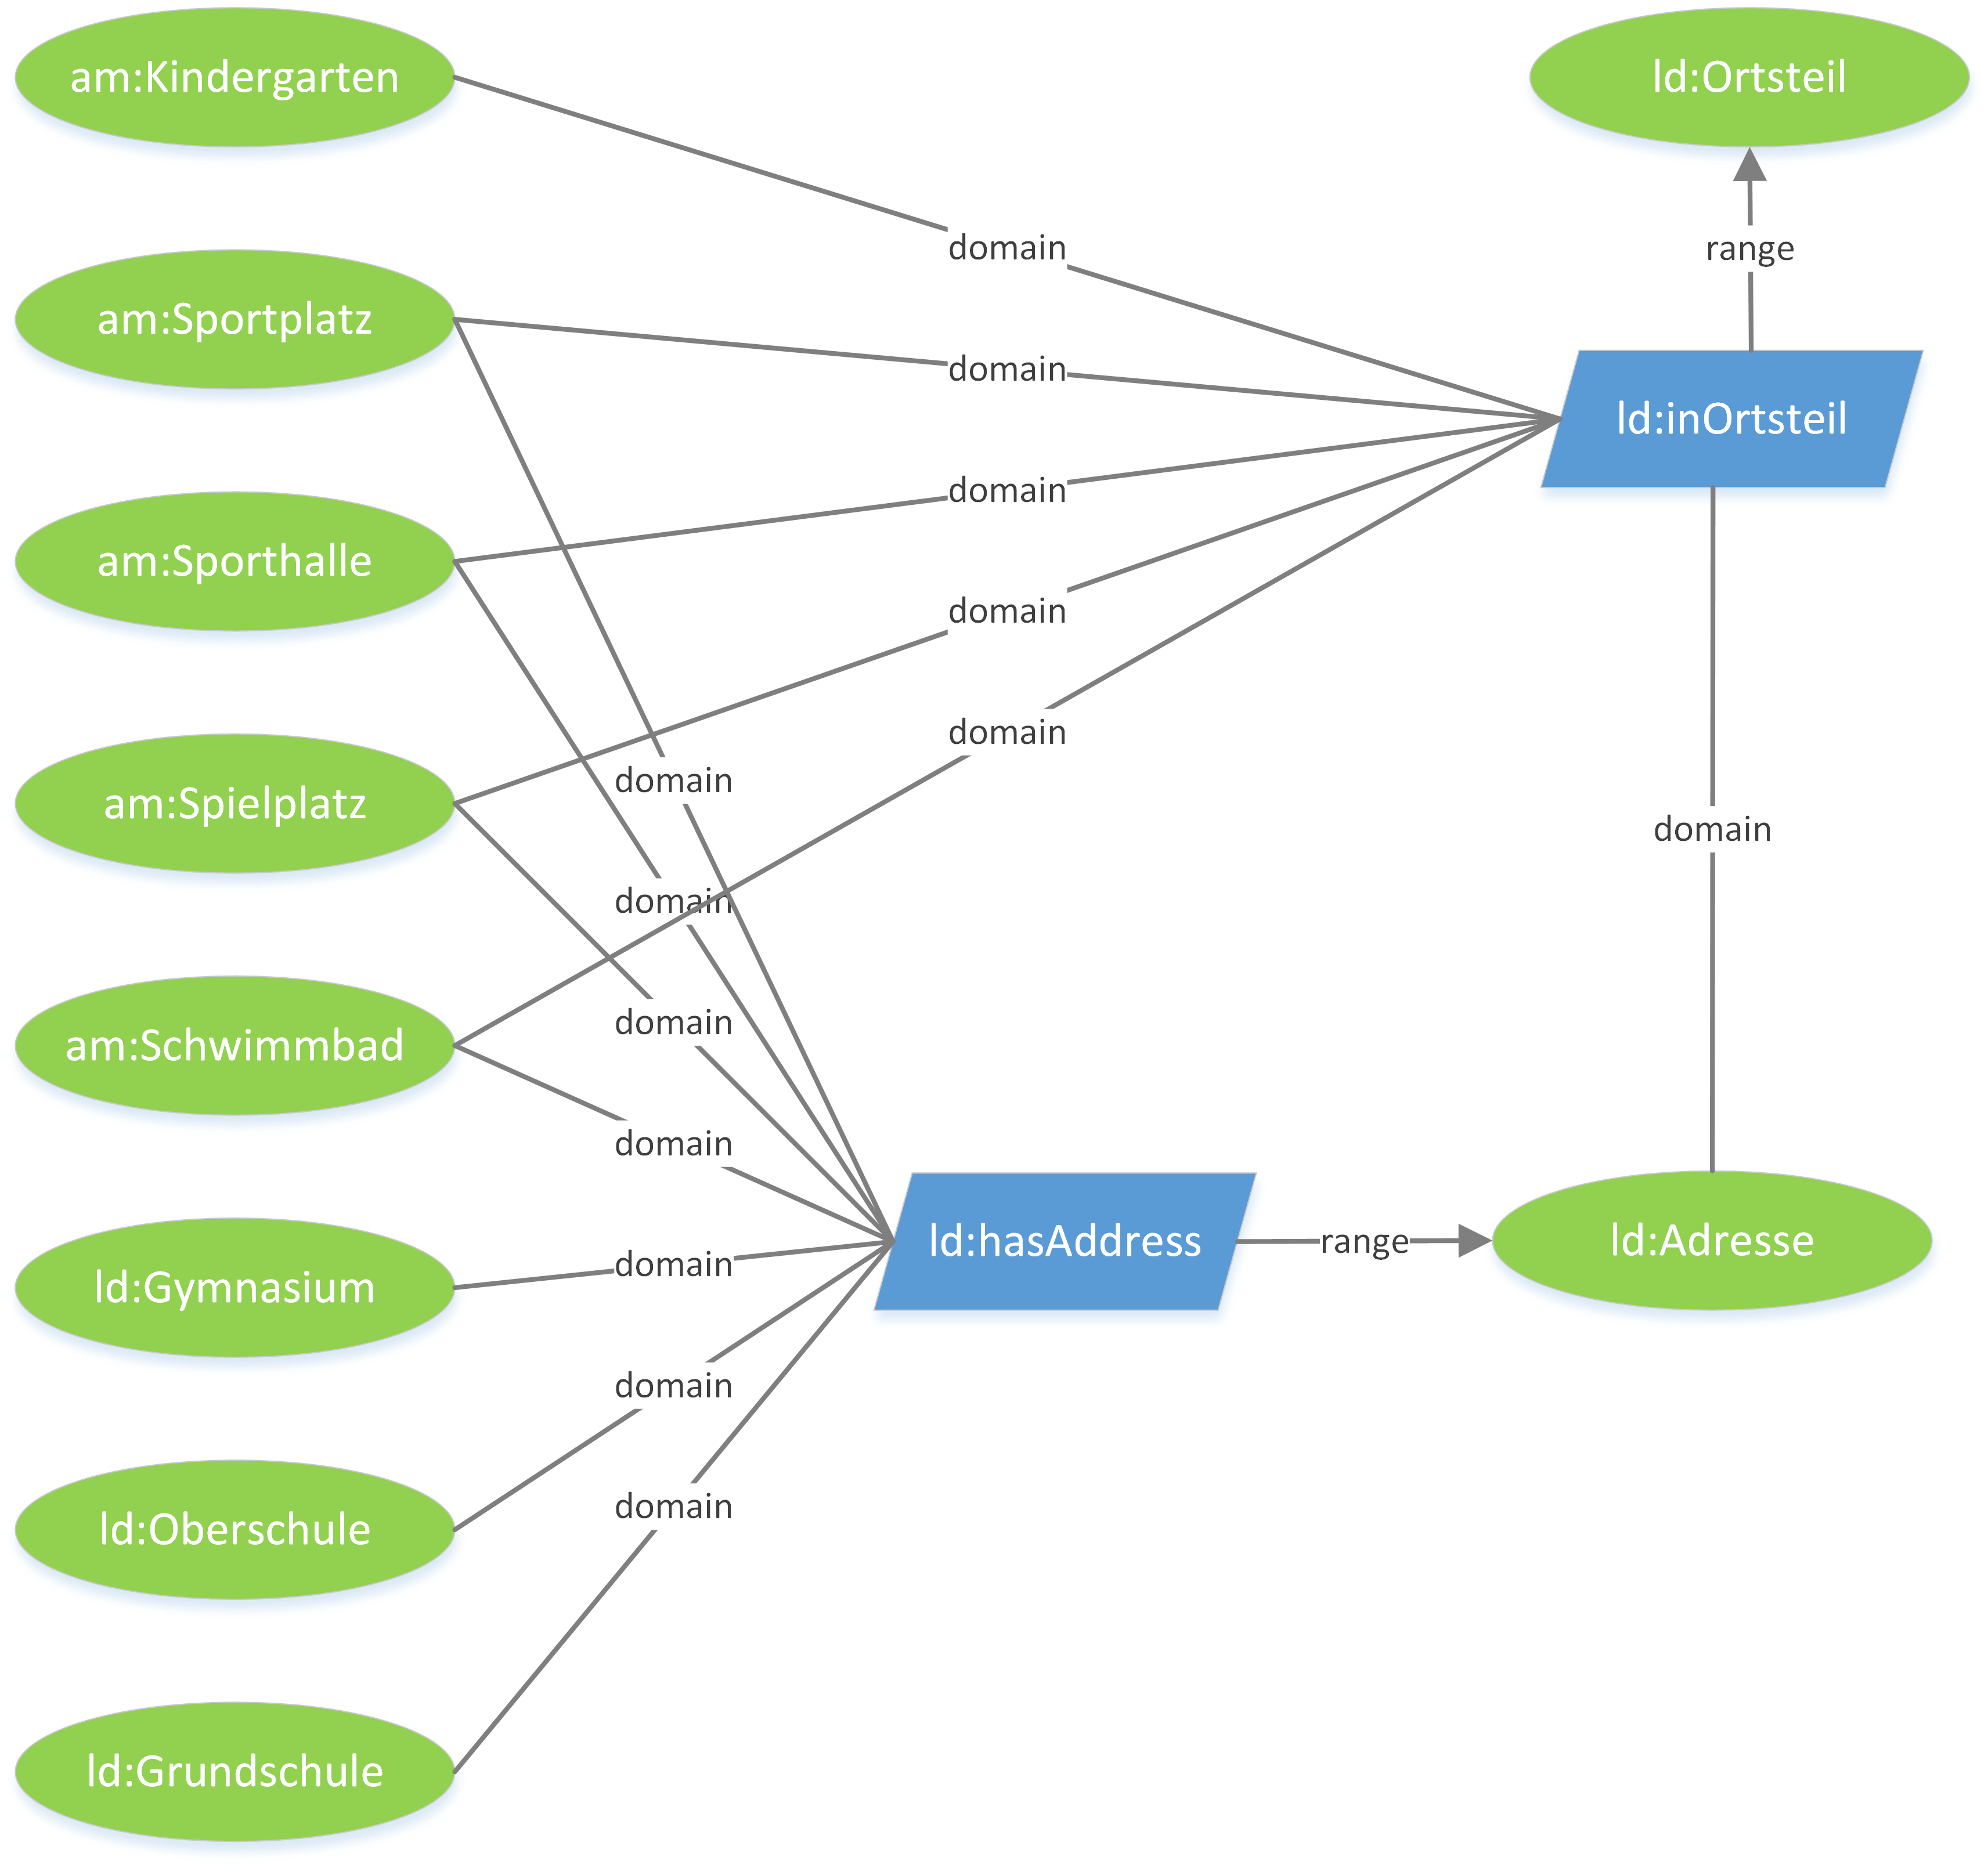
\includegraphics[width=0.95\textwidth]{schema.png}
 \caption{RDF-Schema}
 \label{figure_schema}
\end{figure}


Um die Fragestellungen zu beantworten ist es notwendig von den jeweiligen Einrichtung eine Verbindung zu dem Stadtteil herzustellen, in dem sie sich befindet. In den Klassen für Schule, Kindergarten, Spielplatz, Schwimmbad, Sporthalle und Sportplatz existiert eine direkte Verbindung über die \textit{ld:inOrtsteil} Property. Dagegen haben die Klassen der drei Schularten keine direkte Verknüpfung zu einem Stadtteil. Diese muss daher über die Adresse und die Property \textit{ld:hasAddress} hergestellt werden, da jede Adresse einem Ortsteil zugeordnet ist. Diese sind bei allen Klassen gleich, bis auf die der Schulen, da bei diesem der Stadtteil über die Adresse verknüpft werden muss. 



\section{Anfrage an die Forschungswissensbasis}

\subsection{SPARQL-Anfrage}
In einer SPARQL-Anfrage sollen nun alle Einrichtungen in den Stadtteilen gezählt werden. Dazu wird für jeden Klasse eine Abfrage benötigt, in der alle Objekte der Klasse mit dem dazugehörigen Stadtteil abgerufen werden. Anschließend wird über die Stadtteile gruppiert (\texttt{GROUP BY}) und dann die Anzahl mit  \texttt{COUNT()} gezählt. In Listing \ref{list:sparql1} und Listing \ref{list:sparql2} ist der Unterschied zu sehen, ob die Zuordnung zu einem Stadtteil direkt über die Property\textit{ld:inOrtsteil} oder erst über die Adresse hergestellt wird.


\lstset{
language=c,
frame=single,
xrightmargin=.5em,
xleftmargin=.5em
}


\begin{minipage}{.5\textwidth}
\begin{lstlisting}[caption={Abfrage direkt über ld:inOrtsteil}, label={list:sparql1}]
SELECT ?ort (count(?y) as ?kiga)
WHERE {
    ?y a am:Kindergarten .
    ?y ld:inOrtsteil ?ort . 
}
GROUP BY ?ort
~
\end{lstlisting}
\end{minipage}%
\begin{minipage}{.5\textwidth}
\begin{lstlisting}[caption={Abfrage über ld:hasAddress}, label={list:sparql2}]
SELECT ?ort (count(?g) as ?gym )
WHERE {
    ?g rdf:type ld:Gymnasium.
    ?g ld:hasAddress ?a.
    ?a ld:inOrtsteil ?ort.
}
GROUP BY ?ort
\end{lstlisting}
\end{minipage}


Um diese Zählung für alle Klassen gleichzeitig durchzuführen, werden diese einzelnen Abfragen in einer Abfrage  geschachtelt. In der äußeren Abfrage werden dann zuerst alle Ortsteile mit ihren Namen abgerufen. Da nicht jede Einrichtung in jedem Stadtteil vorhanden ist, dürfen nicht vorhandene Einträge auch nicht entfernt werden. In SQL würde das einem \texttt{LEFT OUTER JOIN} entsprechen. In SPARQL wird diese Funktionalität mit dem Schlüsselwort \texttt{OPTIONAL} eingesetzt. Der fehlende Wert bleibt somit in der entsprechenden Spalte leer und muss für eine spätere Auswertung mit 0 ersetzt werden. Durch die fehlenden Felder ist eine Aggregation der Werte in der äußeren Abfrage jedoch nicht mehr möglich. In Listing \ref{list:sparql} ist eine gekürzte Version der finalen SPARQL-Abfrage an die Wissenbasis abgebildet.

\begin{lstlisting}[caption={SPARQL-Anfrage}, label={list:sparql}]
PREFIX am: <http://www.imn.htwk-leipzig.de/~amuelle3/Data/Model/>
PREFIX ld: <http://leipzig-data.de/Data/Model/>
PREFIX rdfs: <http://www.w3.org/2000/01/rdf-schema\#>
PREFIX rdf: <http://www.w3.org/1999/02/22-rdf-syntax-ns\#>

SELECT ?Ort ?grund ?gym ?ober ?kiga ?spielplatz ?schwimmbad ?sportplatz ?sporthalle
where
{
  ?ort a ld:Ortsteil .
  ?ort rdfs:label ?Ort .
  
  OPTIONAL {
    select ?ort (count(?g) as ?gym )
    where {
        ?g rdf:type ld:Gymnasium.
        ?g ld:hasAddress ?a.
        ?a ld:inOrtsteil ?ort.
    }
    GROUP BY ?ort
  }
  OPTIONAL {
    SELECT ?ort (count(?y) as ?kiga)
    WHERE {
        ?y a am:Kindergarten .
        ?y ld:inOrtsteil ?ort . 
    }
    GROUP BY ?ort  
  }
}
\end{lstlisting}

Die vollständige SPARQL-Abfrage kann in dem veröffentlichten GitHub-Repository\footnote{siehe \url{https://github.com/muexx/sematic-web}} eingesehen werden.


\subsection{Ergebnis der Anfrage}
Das Ergebnis der Anfrage ist eine Tabelle mit allen Stadtteilen in der ersten Spalte und der jeweiligen Anzahl der vorhandenen Einrichtungen in den folgenden Spalten. Das Resultat wurde zur Auswertung als CSV-Datei exportiert und leere Spalten mit Null aufgefüllt. Anschließend wurde die Anzahl der Einrichtungen pro Stadtteil aufsummiert, um das Ergebnis auf die Fragestellung zu erhalten.


In Tabelle \ref{ergebnisse1} sind die Stadtteile mit den meisten kinderfreundlichen Einrichtung zu sehen. Tabelle \ref{ergebnisse2} zeigt die Stadtteile mit den wenigsten kinderfreundlichen Einrichtung. 

\newcolumntype{N}{>{\scriptsize}1}
\newcolumntype{V}[1]{>{\scriptsize\raggedright\hspace{0pt}}p{#1}}

\begin{table}[h, label={ergebisse1}]
\caption{familienfreundlichste Stadtteile}
\begin{tabular} {@{}*{11}{l}@{}}
\toprule
\# & 
Stadtteil & 
\multicolumn{1}{V{3em}@{}}{Grund-schulen} & 
\multicolumn{1}{V{3em}@{}}{Gym-nasien} & 
\multicolumn{1}{V{3em}@{}}{Ober-schulen} & 
\multicolumn{1}{V{3em}@{}}{Kinder-gärten} & 
\multicolumn{1}{V{3em}@{}}{Spielplätze} & 
\multicolumn{1}{V{3.5em}@{}}{Schwimm-bäder} & 
\multicolumn{1}{V{3em}@{}}{Sport-plätze} & 
\multicolumn{1}{V{3em}@{}}{Sport-hallen} & 
$\Sigma$ \\

\cmidrule(r){1-1}\cmidrule(lr){2-2}\cmidrule(lr){3-10}\cmidrule(l){11-11}
1 & \multicolumn{1}{V{5em}@{}}{Reudnitz-Thonberg} & 2 & 1 & 1 & 8 & 14 & 0 & 1 & 1 & 28 \\
2 & \multicolumn{1}{V{5em}@{}}{Stötteritz ~~~~~~~~~~} & 1 & 1 & 0 & 8 & 13 & 2 & 1 & 2 & 28 \\
3 & \multicolumn{1}{V{5em}@{}}{Engelsdorf ~~~~~~~~~~~~} & 1 & 1 & 0 & 6 & 15 & 0 & 1 & 0 & 24 \\
4 & \multicolumn{1}{V{5em}@{}}{Zentrum-Südost} & 2 & 1 & 1 & 12 & 7 & 1 & 0 & 0 & 24 \\
5 & \multicolumn{1}{V{5em}@{}}{Neustadt-Neuschönefeld} & 3 & 0 & 0 & 8 & 11 & 0 & 0 & 1 & 23 \\
6 & \multicolumn{1}{V{5em}@{}}{Paunsdorf} & 3 & 0 & 1 & 10 & 5 & 1 & 3 & 0 & 23 \\
\bottomrule
\end{tabular}
\label{ergebnisse1}
\end{table}

\begin{table}[h]
\caption{familienUNfreundlichste Stadtteile}
\begin{tabular} {@{}*{11}{l}@{}}
\toprule
\# & 
Stadtteil & 
\multicolumn{1}{V{3em}@{}}{Grund-schulen} & 
\multicolumn{1}{V{3em}@{}}{Gym-nasien} & 
\multicolumn{1}{V{3em}@{}}{Ober-schulen} & 
\multicolumn{1}{V{3em}@{}}{Kinder-gärten} & 
\multicolumn{1}{V{3em}@{}}{Spielplätze} & 
\multicolumn{1}{V{3.5em}@{}}{Schwimm-bäder} & 
\multicolumn{1}{V{3em}@{}}{Sport-plätze} & 
\multicolumn{1}{V{3em}@{}}{Sport-hallen} & 
$\Sigma$ \\

\cmidrule(r){1-1}\cmidrule(lr){2-2}\cmidrule(lr){3-10}\cmidrule(l){11-11}
63 & \multicolumn{1}{V{5em}@{}}{Grünau-Siedlung} & 0 & 0 & 0 & 0 & 1 & 0 & 0 & 0 & 1 \\
62 & \multicolumn{1}{V{5em}@{}}{Baalsdorf ~~~~~~~~~~} & 0 & 0 & 0 & 1 & 2 & 0 & 0 & 0 & 3 \\
61 & \multicolumn{1}{V{5em}@{}}{Heiterblick ~~~~~~~~~~} & 0 & 1 & 0 & 1 & 2 & 0 & 0 & 0 & 4 \\
60 & \multicolumn{1}{V{5em}@{}}{Miltitz ~~~~~~~~~~~~~} & 1 & 0 & 0 & 1 & 1 & 0 & 1 & 0 & 4 \\
59 & \multicolumn{1}{V{5em}@{}}{Meusdorf ~~~~~~~~~~} & 1 & 0 & 0 & 1 & 2 & 0 & 0 & 1 & 5 \\ 
58 & \multicolumn{1}{V{5em}@{}}{Zentrum ~~~~~~~~~~} & 0 & 0 & 0 & 0 & 2 & 0 & 0 & 3 & 5 \\
\bottomrule
\end{tabular}
\label{ergebnisse2}
\end{table}


\section{Interpretation und Zusammenfassung}
Wie aus den Ergebnistabellen abzulesen ist gibt es deutliche Unterschiede zwischen den Stadtteilen von Leipzig bei der Anzahl der kinderfreundlichen Einrichtungen. Dabei ist jede Kategorie der Einrichtungen gleich gewichtet, was eventuell nicht die Anforderungen der meisten Familien widerspiegelt. Aus dieser Überlegung heraus wäre es denkbar, die Ergebnisse zu personalisieren und den verschiedenen Kategorien eine andere Gewichtung zu geben. Zum Beispiel würde eine Familie mit Kindern, die bereits die Grundschule besuchen, der Kategorie der Kindergärten ein geringeres Gewicht geben, als der Kategorie der Gymnasien und Oberschulen, auf welche die Kinder in Zukunft gehen werden.
Um eine solche Gewichtung zu realisieren, würde die Anzahl der entsprechenden Kategorien mit dem jeweiligen Gewicht multipliziert werden. Das würde das Gesamtergebnis jedes Stadtteils verändern und eine neue Sortierung erfordern.

Ob dies jedoch trotz dieser Anpassung als eindeutiges Maß der Kinderfreundlichkeit eines Stadtteils herangezogen werden kann, ist zu bezweifeln. Beispielsweise wurde bei der Fragestellung die Größe eines Stadtteiles komplett vernachlässigt. Auch die beschränkte Auswahl der acht verschiedenen Einrichtungen ist unzureichend, um die Fragestellungen zu beantworten. Mögliche Faktoren, die eventuell aussagekräftiger seien könnten, wäre der Altersdurchschnitt und der Anteil der bereits ansässigen Familien mit Kindern.






\end{document}
